\usepackage{graphicx}
\usepackage{comment}
\usepackage[font=scriptsize]{caption}
\usepackage{subcaption} 


 
\newenvironment{theorem}[2][Twierdzenie]{\begin{trivlist}
\item[\hskip \labelsep {\bfseries #1}\hskip \labelsep {\bfseries #2.}]}{\end{trivlist}}
\newenvironment{question}[2][Pytanie]{\begin{trivlist}
\item[\hskip \labelsep {\bfseries #1}\hskip \labelsep {\bfseries #2.}]}{\end{trivlist}}
\newenvironment{hypothesis}[2][Hipoteza]{\begin{trivlist}
\item[\hskip \labelsep {\bfseries #1}\hskip \labelsep {\bfseries #2.}]}{\end{trivlist}}
\newenvironment{lemma}[2][Lemat]{\begin{trivlist}
\item[\hskip \labelsep {\bfseries #1}\hskip \labelsep {\bfseries #2.}]}{\end{trivlist}}
\newenvironment{exercise}[2][Ćwiczenie]{\begin{trivlist}
\item[\hskip \labelsep {\bfseries #1}\hskip \labelsep {\bfseries #2.}]}{\end{trivlist}}
\newenvironment{reflection}[2][Uwaga]{\begin{trivlist}
\item[\hskip \labelsep {\bfseries #1}\hskip \labelsep {\bfseries #2.}]}{\end{trivlist}}
\newenvironment{proposition}[2][Założenie]{\begin{trivlist}
\item[\hskip \labelsep {\bfseries #1}\hskip \labelsep {\bfseries #2.}]}{\end{trivlist}}
\newenvironment{corollary}[2][Wniosek]{\begin{trivlist}
\item[\hskip \labelsep {\bfseries #1}\hskip \labelsep {\bfseries #2.}]}{\end{trivlist}}

\begin{document}

\title{Implementacja protokołów populacyjnych\\oraz testy wydajnościowe}
\author{Grams, Stanisław\\Jezierski, Maciej\\Korczakowski, Juliusz\\ MFI UG\\Algorytmy Numeryczne}

\maketitle
\section {Operacje na macierzach}
\subsection{O implementacji}
Program \textit{„protocols”} został napisany w języku C++ z użyciem bibliotek z standardu C++. 
Wyniki działania programu zapisywane są do poszczególnych plików \textit{*.csv}.
\subsection{Zaimplementowane algorytmy}
\begin{itemize}
	\item (PG - Partial Gauss) Algorytm Gaussa z częściowym wyborem elementu
	\item (PGO - Partial Gauss Optimised) Algrotym Gaussa z optymalizacją dla macierzy rzadkich
	\item Algroytm Jacobiego
	\item Algorytm Jacobiego w wersji iteracyjnej
	\item Algorytm Gaussa-Seidela
	\item Algorytm Gaussa-Seidela z postacią iteracyjną
	\item Metoda Monte Carlo
\end{itemize}

\section{Implementacja i jej poprawność}
\subsection{Generowanie układu równań dla danej liczby agentów}
Generowanie układu równań dla danego $N$ odbywa się w sposób następujący:
\begin{enumerate}
	\item Określenie wszystkich możliwych przypadków (ilość agentów $\#Y$ oraz ilość agentów $\#N$),
	\item Wyliczenie wszystkich możliwych kombinacji bez powtórzeń za pomocą Symbolu Newtona ${{N} \choose {2}}$,
	\item Wygenerowanie równań dla poszczególnych przypadków,
	\item Osadzenie równań w macierzy,
	\item Wypełnienie wektora $B$ zerami.
\end{enumerate}
\subsection{Prawidłowość implementacji}
By zweryfikować poprawność implementacji zarówno generowania macierzy jak i obliczania stworzonego w ten sposób układu równań, wszelkie obliczenia porównywane były z wyliczonym metodą Monte Carlo. Poniższy wykres obrazuje dokładność wszystkich zaimplementowanych algorytmów względem metody Monte Carlo na podstawie, którego można wnioskować o poprawności zaimplementowanych metod.

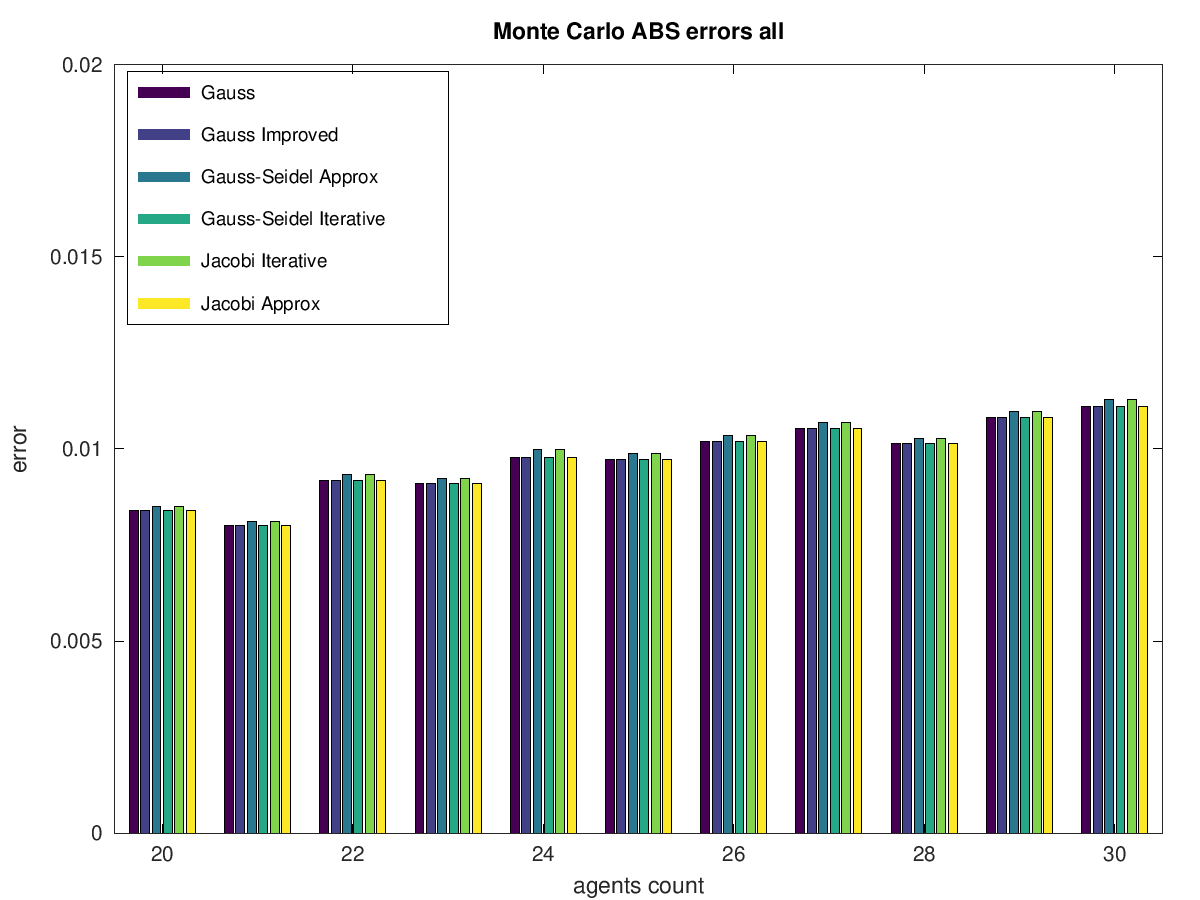
\includegraphics[scale=0.75]{01_abs_all_methods_all_rows.png}

\section{Analiza wyników i wydajność zaimplementowanych algorytmów}

\subsection{Analiza wyników}
\subsubsection{Gauss oraz Gauss z optymalizacją dla macierzy rzadkich}
Przeanalizujmy poniższy wykres. Wynika z niego jednoznacznie, że optymalizacja nie wpływa na dokładność. Wyraźnie widać, że na praktycznie całej długości wykresu błąd wynosi 0 z rzadkimi wyjątkami na korzyść metody zoptymalizowanej.
\begin{figure}[h]
\centering
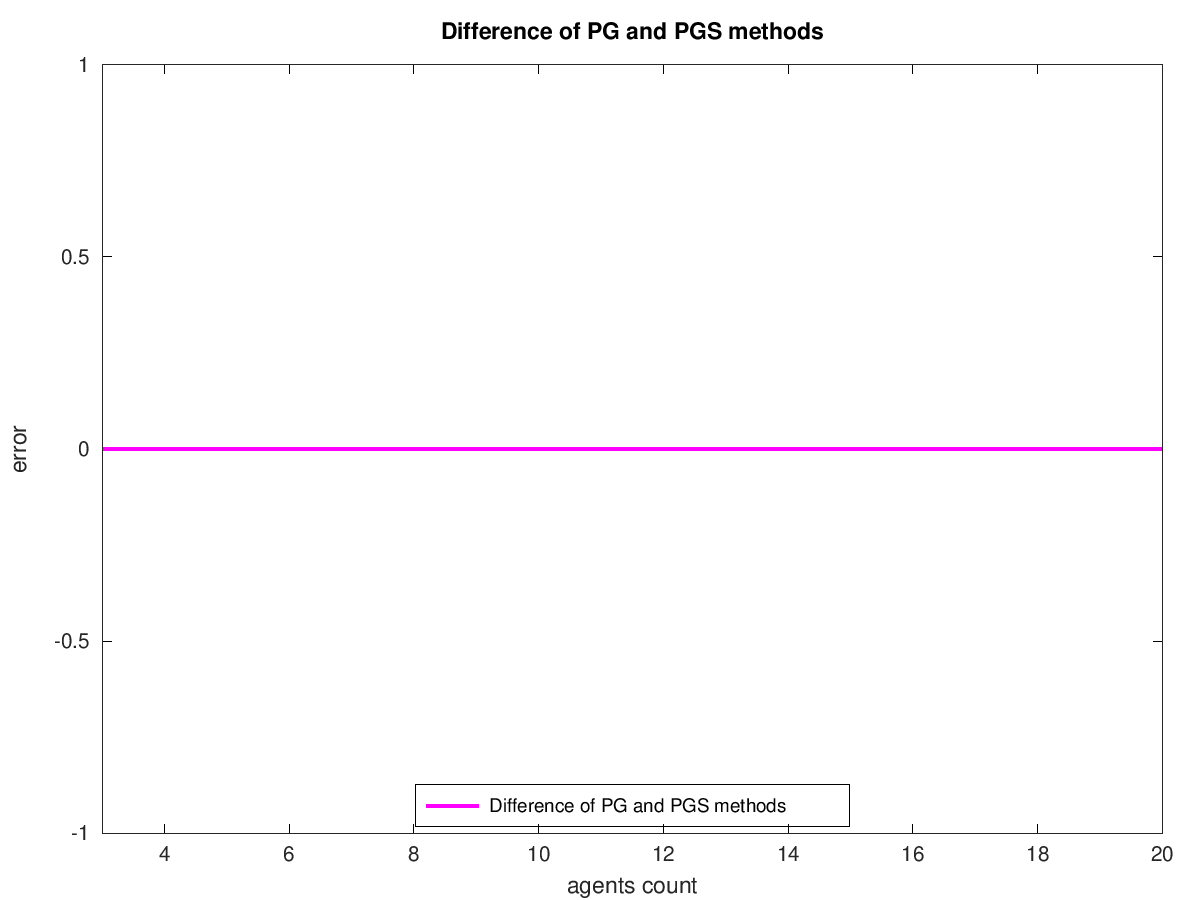
\includegraphics[scale=0.43]{07_abs_gauss_and_gauss_optimized_all_rows.png}
\end{figure}

\subsubsection{Algorytmy iteracyjne}
Obie zaimplementowane przez nasz zespół metody oferują przyzwoitą dokłądność jednak poniższe wykresy pozwalają wyciągnąć wniosek mówiący, że medoda Gaussa-Seidela jest dokładniejsza. Warto także zaznaczyć, że metody iteracyjne cechują się jednak najgorszymi wynikami zarówno w klasie dokładności jak i czasu wykonania.

\begin{figure}[h]
\centering
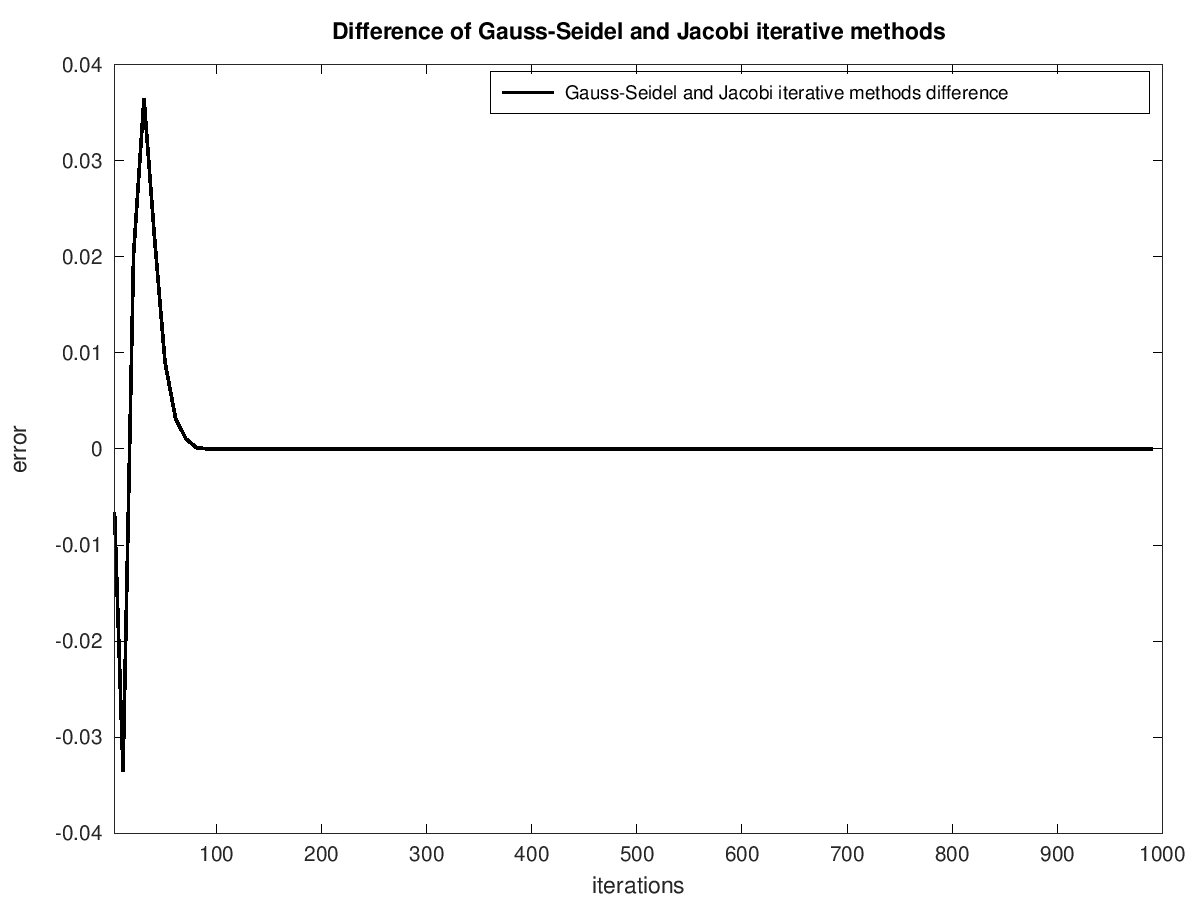
\includegraphics[scale=0.45]{03_abs_iterative_methods_all_rows.png}
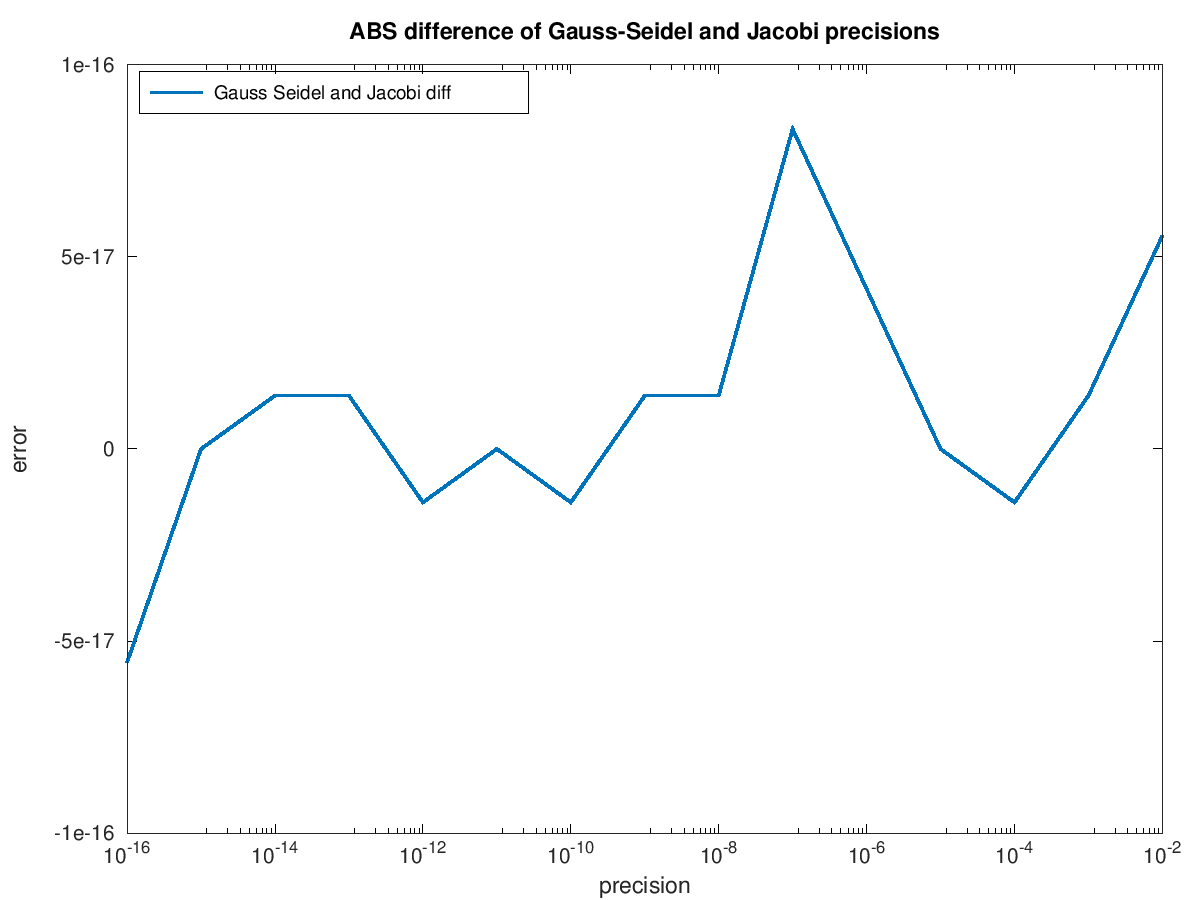
\includegraphics[scale=0.45]{05_abs_precision_methods_all_rows.png}
\end{figure}
\subsection {Wydajność}
\subsubsection{Wydajność względem wielkości planszy}
Analizując poniższe wykresy można wyciągnąć następujące wnioski:\\
1. Pod względem błędów obliczeń metody Gaussa oraz Gaussa z ulepszeniem dla macierzy rzadkich zdecydowanie wygrywają z innymi algorytmami oferując idealnie taką samą, wysoką dokładność.\\
2. Ze wzglęgu na swoją specyfikacje metoda Gaussa z ulepszeniem dla macierzy rzadkich wygrywa z klasyczną wersją tej metody pod względem czasu wykonania.\\
\\
Powyższe wnioski wyraźnie wskazują, że w klasie wydajności względem wielkości planszy jako optymalny wybór należy wskazać metodę Gaussa z ulepszeniem dla macierzy rzadkich.
\begin{figure}[h]
\centering
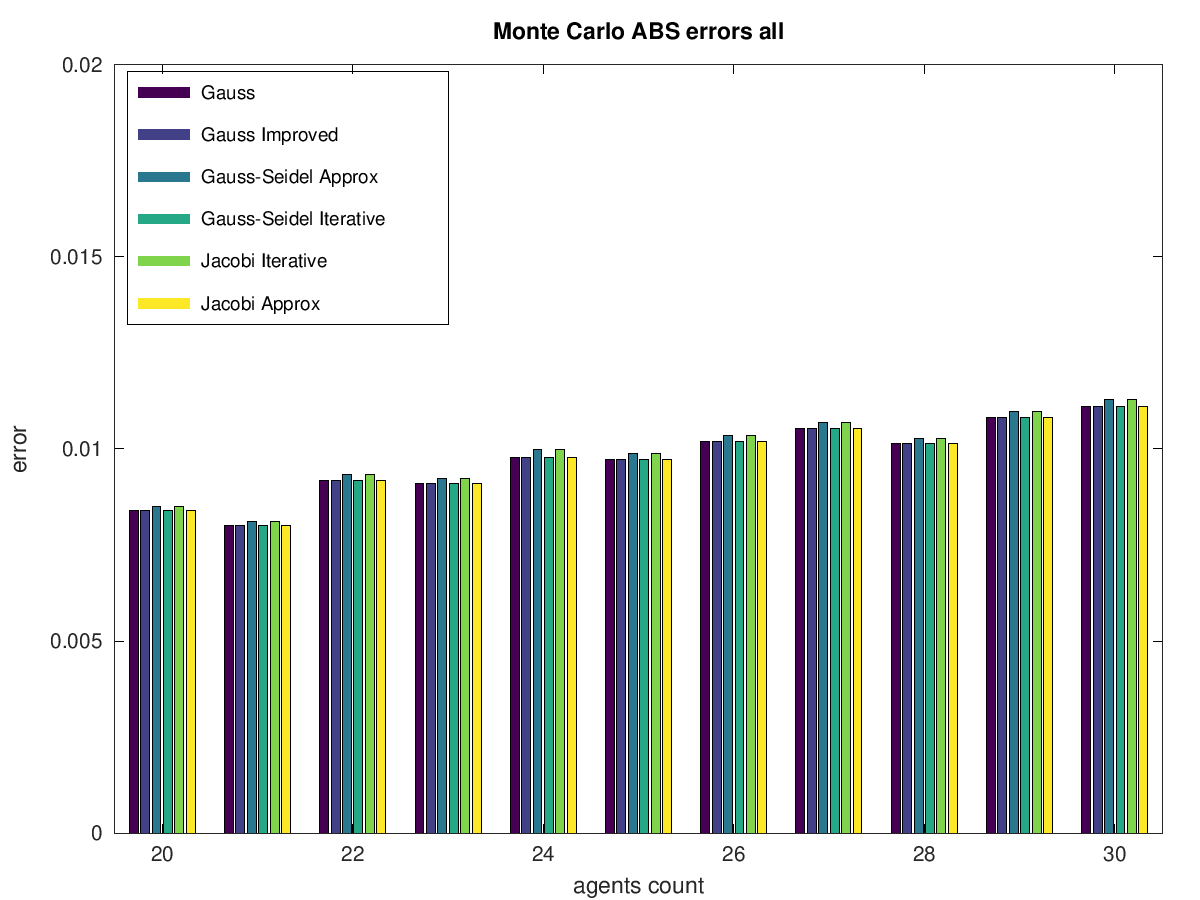
\includegraphics[scale=0.45]{01_abs_all_methods_all_rows.png}
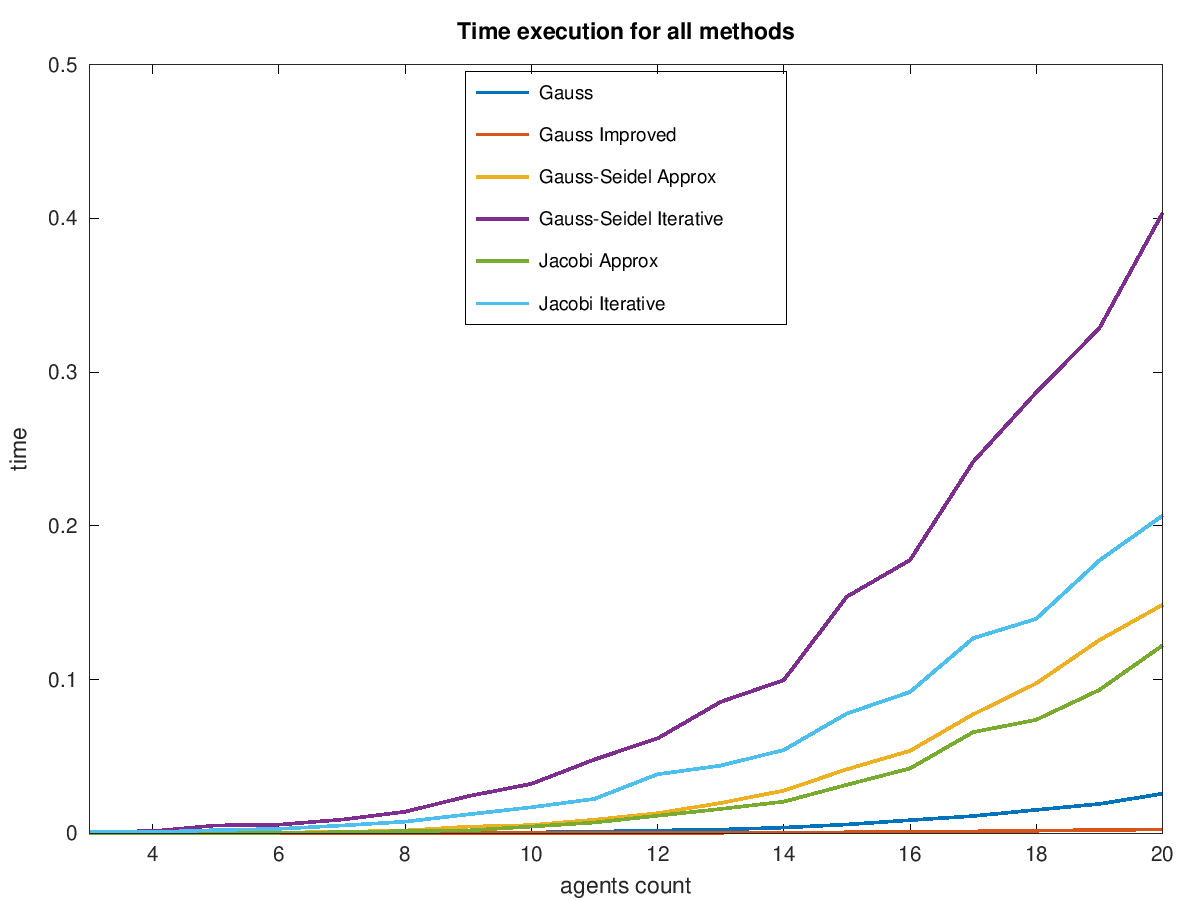
\includegraphics[scale=0.45]{02_time_execution_all_methods.png}
\end{figure}
\newpage

\subsubsection{Wydajność względem zadanej dokładności}
\begin{figure}[h]
\centering
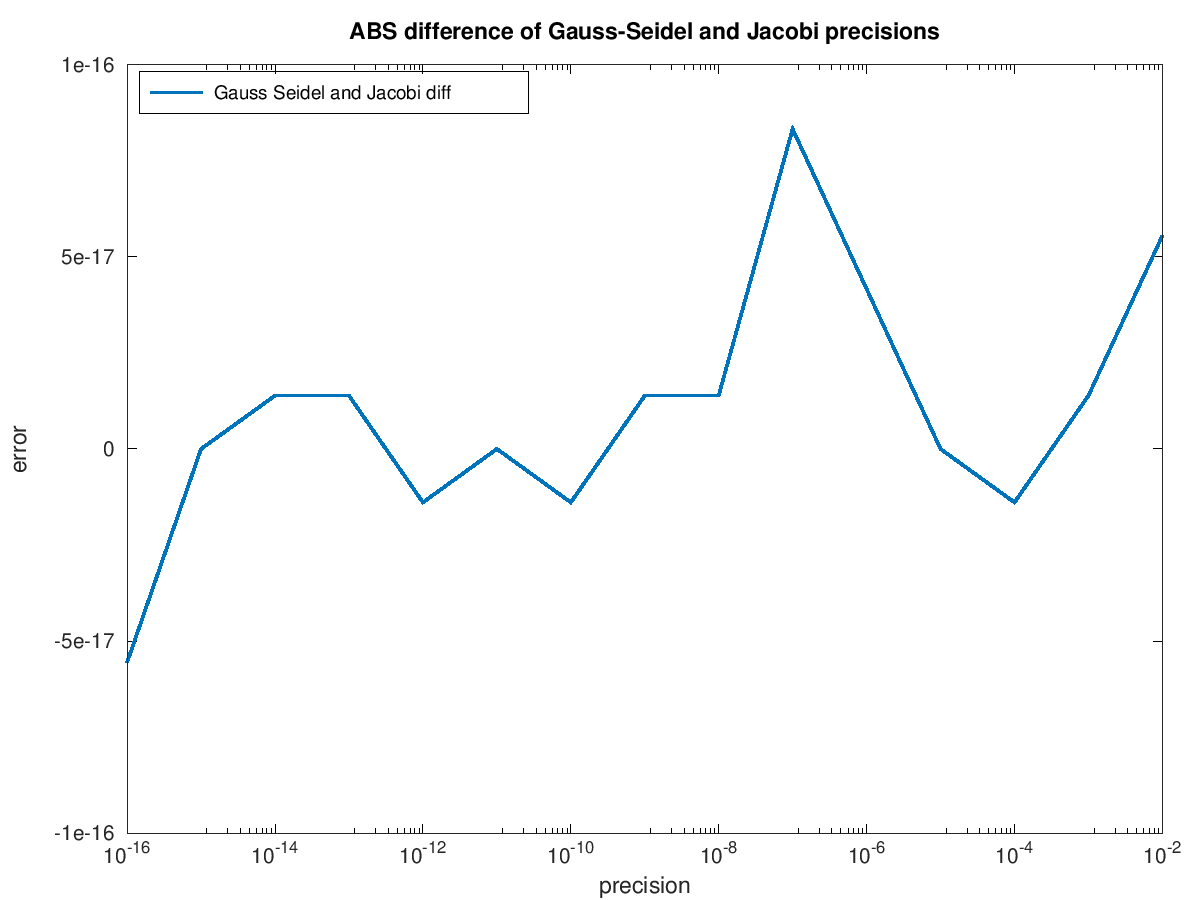
\includegraphics[scale=0.45]{05_abs_precision_methods_all_rows.png}
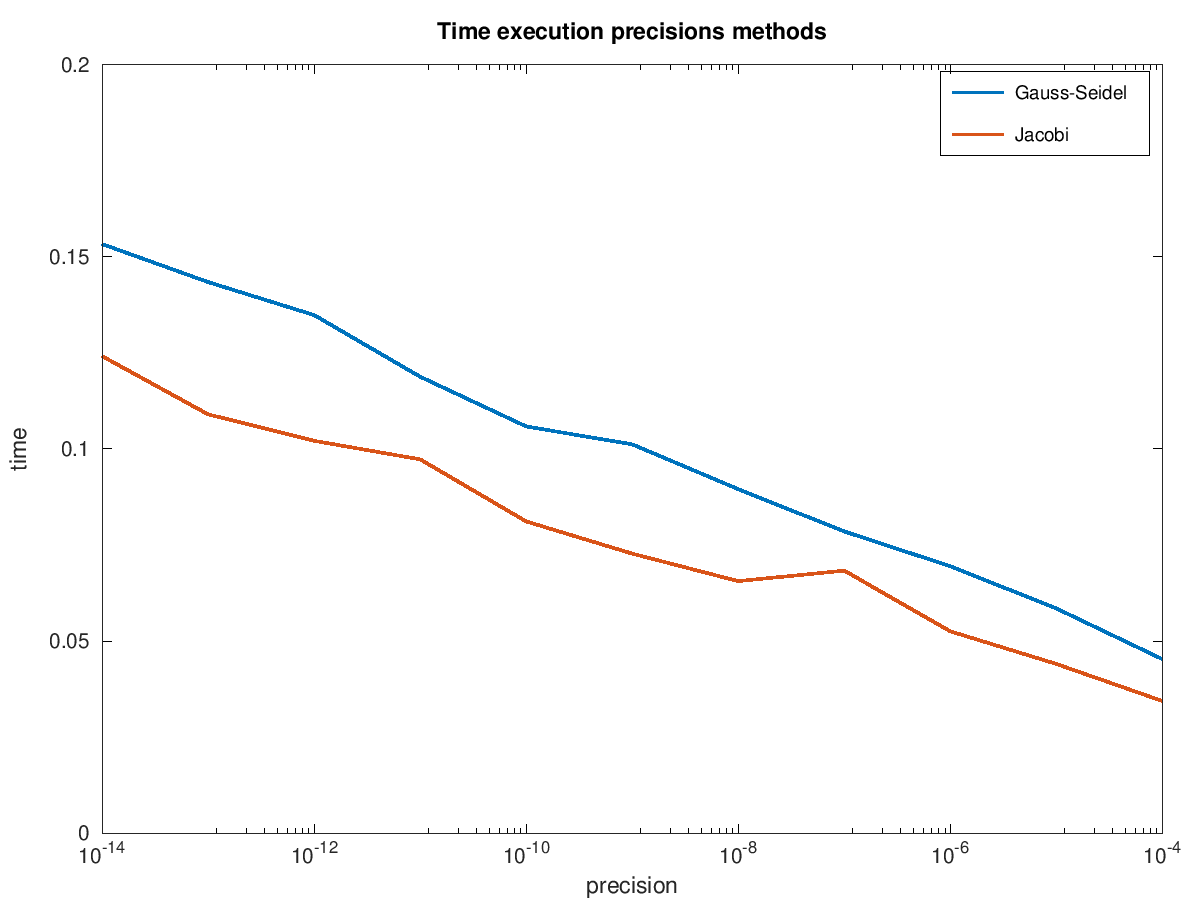
\includegraphics[scale=0.45]{06_time_precision_methods_all_rows.png}
\end{figure}
W przypadku tego kryterium możemy porównać tylko meody Jacobiego oraz Gaussa-Seidela. Na pierwszym wykresie widzimy różnicę błędów między powyższymi metodami, w tej kategorii zdecydowanie wygrywa metoda Gaussa-Seidela, którego dokładność spada dopiero po zadaniu bardzo wysokiego $\epsilon$ większego niż $10^{-14}$. W kwestii czasu wykonania oba algorytmy plasują się bardzo podobnie, jednak tak jak w poprzednim przypadku w okolicach $\epsilon$=$10^{-14}$ następuje załamanie tym razem jednak na korzyść Gaussa-Seidela.\\
Podsumowując, do pewnej dokładności metoda Gaussa dokładniejsza jednak przekraczając ją zyskuje na prędkości wykonania kosztem dokładności licząc względem metody Jacobiego.

\section{Podział pracy}
\centering
	\begin{tabular}{| p{5cm} | p{5cm} | p{5cm} |}
		\hline
		\textbf{Stanisław Grams} & \textbf{Juliusz Korczakowski} & \textbf{Maciej Jezierski} \\ \hline
		Implementacja algorytmu Gaussa-Seidela& Implementacja algorytmu Jacobiego & Implementacja algorytmu PG oraz PGS  \\ \hline
		 Implementacja symulacji Monte Carlo& Przygotowanie testów i ich uruchomienie &Analiza wykresów oraz przygotowanie sprawozdania \\ \hline
		Implementacja algorytmu generowania macierzy & Przygotowanie wykresów końcowych &Praca nad strukturą projektu\\ \hline
	\end{tabular}
\end{document}
